\documentclass{article}

%% Page Margins %%
\usepackage{geometry}
\geometry{
    top = 0.75in,
    bottom = 0.75in,
    right = 0.75in,
    left = 0.75in,
}

\usepackage{amsmath}
\usepackage{graphicx}
\usepackage{parskip}

\title{Lab 6: Finite State Machines}

% TODO: Enter your name
\author{Your Name}

\begin{document}
\maketitle

\section{Part I}

\begin{enumerate}

\item Complete Table~\ref{t:part1_state_encodings} below.

\begin{table}[ht!]
\caption{State Encodings}
\label{t:part1_state_encodings}
\centering
\begin{tabular}{|l|l|}
\hline
State & Encoding \\ \hline
\end{tabular}
\end{table}

\item Complete Table~\ref{t:part1_encoded_transition_table} below.

\begin{table}[ht!]
\caption{Encoded State Transition Table for Robo-Snail}
\label{t:part1_encoded_transition_table}
\centering
\begin{tabular}{|l|l|l|}
\hline
Current State & W & Next State \\ \hline
\end{tabular}
\end{table}

\item Derive equations for each of your next state outputs below.

\begin{align*}
    S'_0 &= \\
    S'_1 &= \\
    S'_2 &= \\
    S'_3 &= \\
    S'_4 &= \\
    S'_5 &= \\
    S'_6 &= \\
\end{align*}

\item Export the subcircuit schematic as an image and include it in your report.

\begin{figure}[ht!]
    \centering
    % 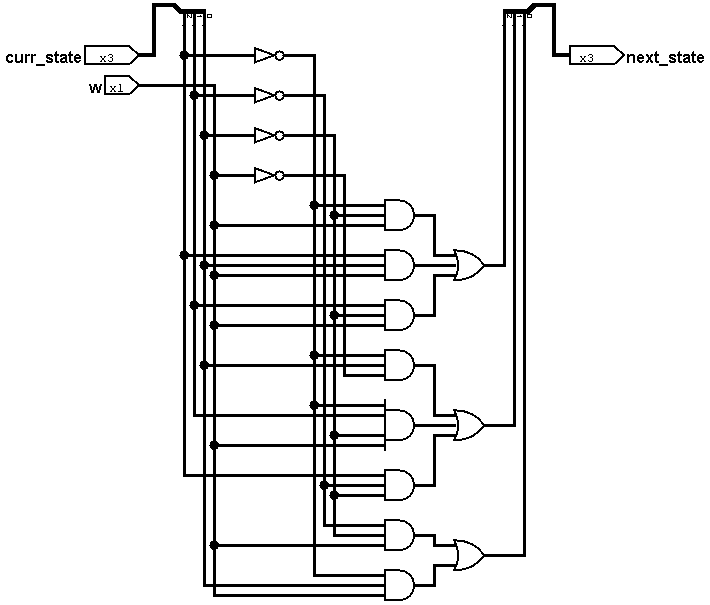
\includegraphics[width=0.3\textwidth]{lab6_part1_next_state.png}
    \caption{A schematic of part1\_state\_table.}
    \label{f:part1_state_table}
\end{figure}

\item Complete Table~\ref{t:part1_output_table} below.

\begin{table}[ht!]
\caption{Encoded Output Table for Robo-Snail}
\label{t:part1_output_table}
\centering
\begin{tabular}{|l|l|}
\hline
State   & Output \\ \hline
\end{tabular}
\end{table}

\item Derive the equation for your output logic below.

$$Z = $$

\item Export the subcircuit schematic as an image and include it in your report.

\begin{figure}[ht!]
    \centering
    % 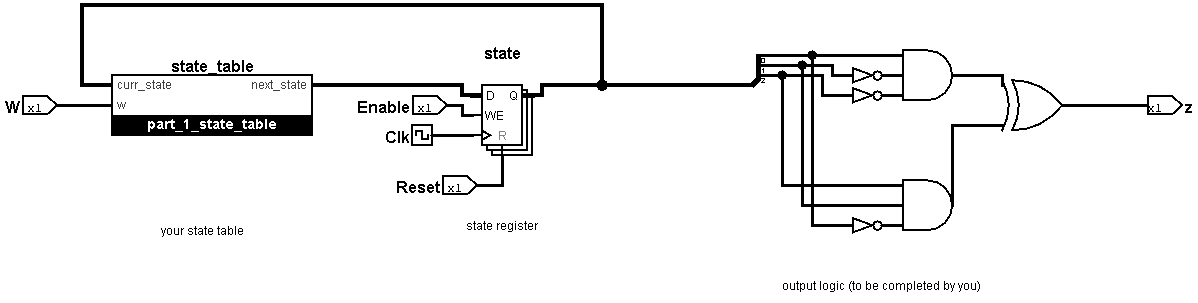
\includegraphics[width=0.5\textwidth]{lab6_part1_output.png}
    \caption{A schematic of part1\_FSM.}
    \label{f:part1_FSM}
\end{figure}
\end{enumerate}

\clearpage
\section{Part II}

\begin{enumerate}
\item Complete Table~\ref{t:part2_encoded_transition_table} below.

\begin{table}[ht!]
\caption{Encoded State Transition Table for Part II}
\label{t:part2_encoded_transition_table}
\centering
\end{table}


\item Draw the state transition diagram and include it in Figure~\ref{f:part2_state_diagram}.

\begin{figure}[ht!]
    \centering
    % 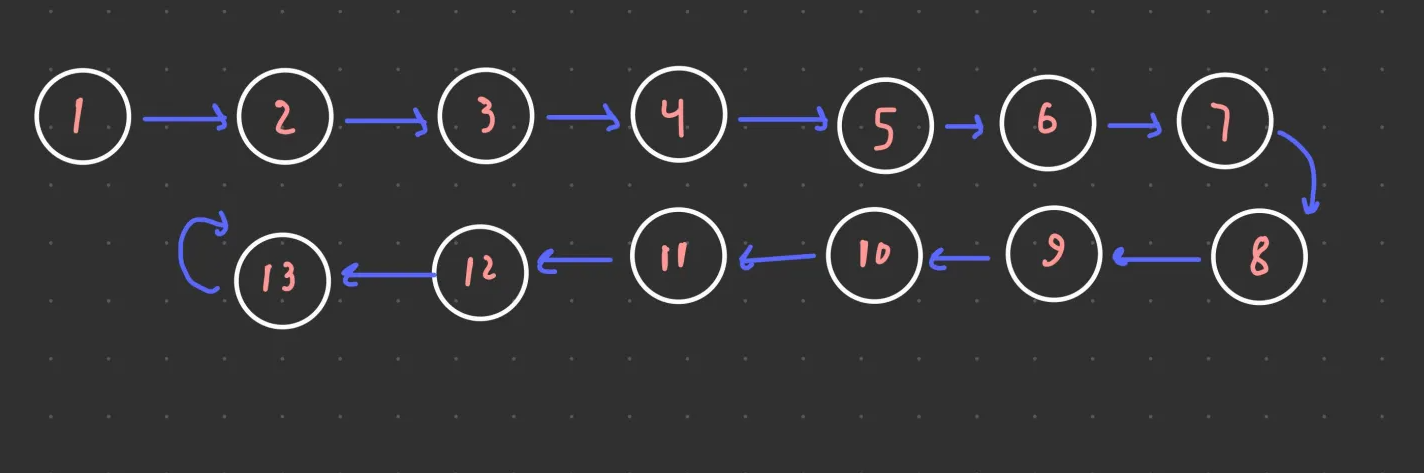
\includegraphics[width=0.3\textwidth]{lab6_part2_state_diagram.png}
    \caption{The state transition diagram for Part II}
    \label{f:part2_state_diagram}
\end{figure}



    \item Simulate your circuit using a variety of input settings.
        
    \begin{figure}[ht!]
    \centering
    % \includegraphics[width=0.65\textwidth]{lab6_part3_testcases.png}
    \caption{Test Case for Part 2.}
    \label{f:part2_testcase 1}
\end{figure}
    \begin{figure}[ht!]
    \centering
    % \includegraphics[width=0.65\textwidth]{lab6_part3_testcases.png}
    \caption{Test Case for Part 2.}
    \label{f:part2_testcase 2}
\end{figure}

\end{enumerate}

\section{Part III}
\begin{enumerate}
    \item Draw a schematic for the datapath of your circuit. It will be similar to the handout. You should show how you will initialize the registers, where the outputs are connected, and include all the control signals that you require.
    
    \item Draw the state diagram that controls your datapath.
    
    \begin{figure}[ht!]
    \centering
    % \includegraphics[width=0.65\textwidth]{lab6_part3_statediagram.png}
    \caption{State diagram that controls the datapath in Part 3.}
    \label{f:part3_statediagram}
\end{figure}

    \item Draw the schematic for your controller module.
    
    \begin{figure}[ht!]
    \centering
    % \includegraphics[width=0.65\textwidth]{lab6_part3_controller.png}
    \caption{Controller Module in Part III.}
    \label{f:part3_controller}
\end{figure}
    
    \item Draw the top-level schematic showing how the datapath and controller are connected as well as the inputs and outputs to your top-level circuit.
    
    \begin{figure}[ht!]
    \centering
    % \includegraphics[width=0.65\textwidth]{lab6_part3_schematics.png}
    \caption{Top level schematics schematic in Part III.}
    \label{f:part3_TLschematics}
\end{figure}
        
    \item Simulate your circuit using a variety of input settings.
        
    \begin{figure}[ht!]
    \centering
    % \includegraphics[width=0.65\textwidth]{lab6_part3_testcases.png}
    \caption{Test Case for Part 3.}
    \label{f:part3_testcase 1}
\end{figure}

        
    \begin{figure}[ht!]
    \centering
    % \includegraphics[width=0.65\textwidth]{lab6_part3_testcases.png}
    \caption{Test Case for Part 3.}
    \label{f:part3_testcase 2}
\end{figure}
\end{enumerate}

\end{document}